% numerics.tex      pdflatex ZhCvGo15
% Diffuse globally, compute locally: a cyclist tale
% Tingnan Zhang, Daniel I. Goldman and Predrag Cvitanovi\'c

%\subsection{Numerical results}
%                         was {Diffusion in the fundamental domain}
%\label{s-numerics}

\begin{table}[htbp]
\hfill
\TZ{2015-10-19}{Do we need this many digits in the table?}
\begin{tabular}{|r|r|r|l|l|}
\hline
$\period{p}$ & \# cycles & $\zeta$(0,0) & $\lambda$ & D \\ \hline\hline
1      & 5      & -0.2169759 & 1.39193 & 0.37795 \\
2      & 10     & -0.0248233 & 1.74541 & 0.23118\\
3      & 33     & -0.0221962 & 1.72235 & 0.25257\\
4      & 108    & -0.0002192 & 1.74450 & 0.24165\\
5      & 373    &  0.0023463 & 1.76079 & 0.24468\\
6      & 1378   &  0.0096330 & 1.75610 & 0.24068\\ \hline\hline
\multicolumn{3}{|l|}{numerical experiment}
                           & 1.760 & 0.25
\\ \hline
\end{tabular}
\caption{\label{TCELL2}
  Results for $w$=0.3. Calculation in FD. Gaspard 1992
  note: ``My numerical estimate for the Lyapunov exponent when $w=0.3$ is
  $\lambda = 1.760 \pm 0.002$, which supports the result of this table.''
}
\end{table}

\begin{figure}[htbp]
  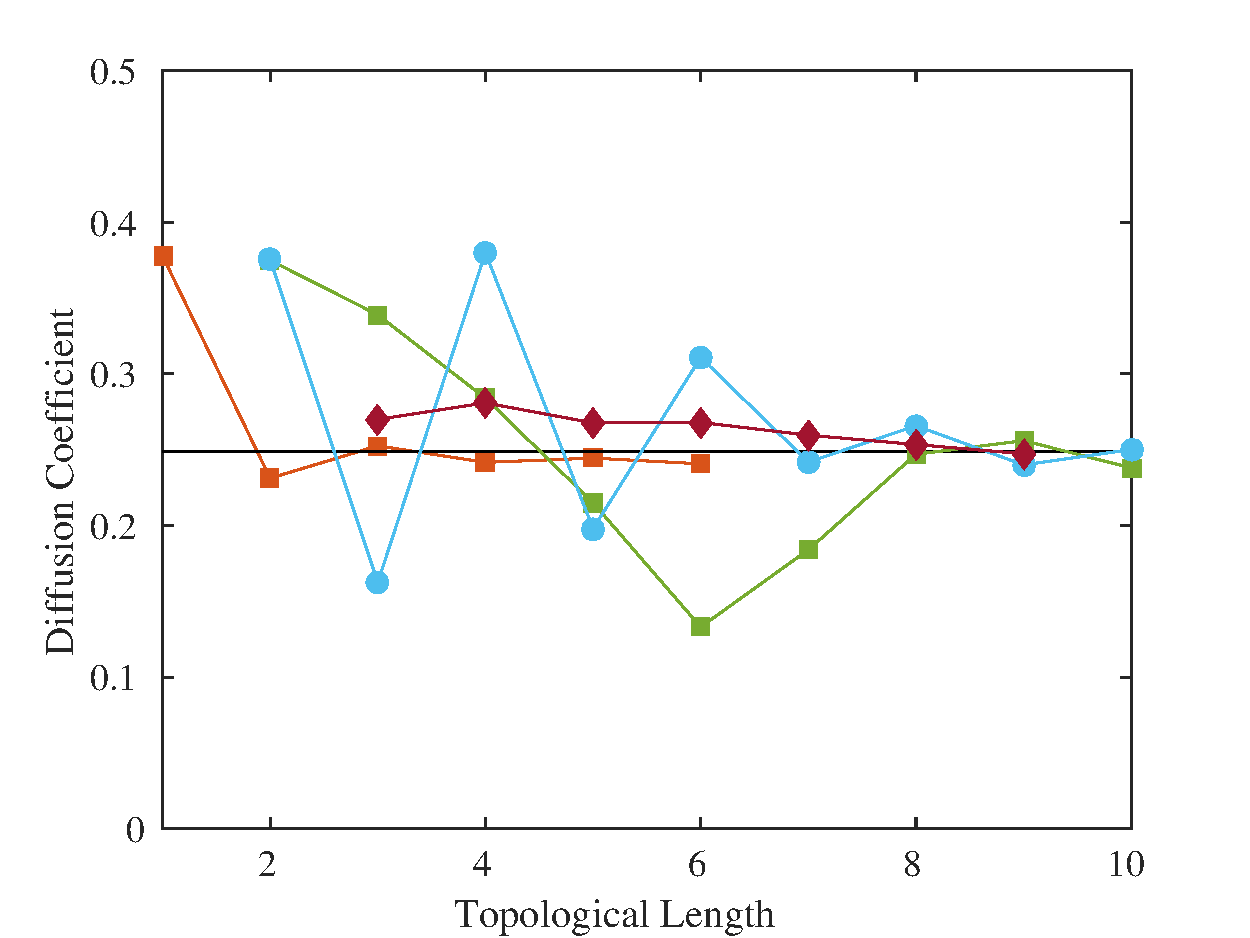
\includegraphics[width=0.45\textwidth]{diffuseCycleExpansionResults}
  \caption[]{\label{fig-convergence}
  The convergence of diffusion coefficients  calculated using cycle
  expansion in elementary cell (green squares),  fundamental
  domain(orange squares). We  also show the convergence of ``periodic
  orbit expansion'' method, with and  without Shanks transformation
  (circles and diamonds) discussed in  \refref{Morriss1994}. Here $w = 0.3$.
  }
\end{figure}

\begin{figure}
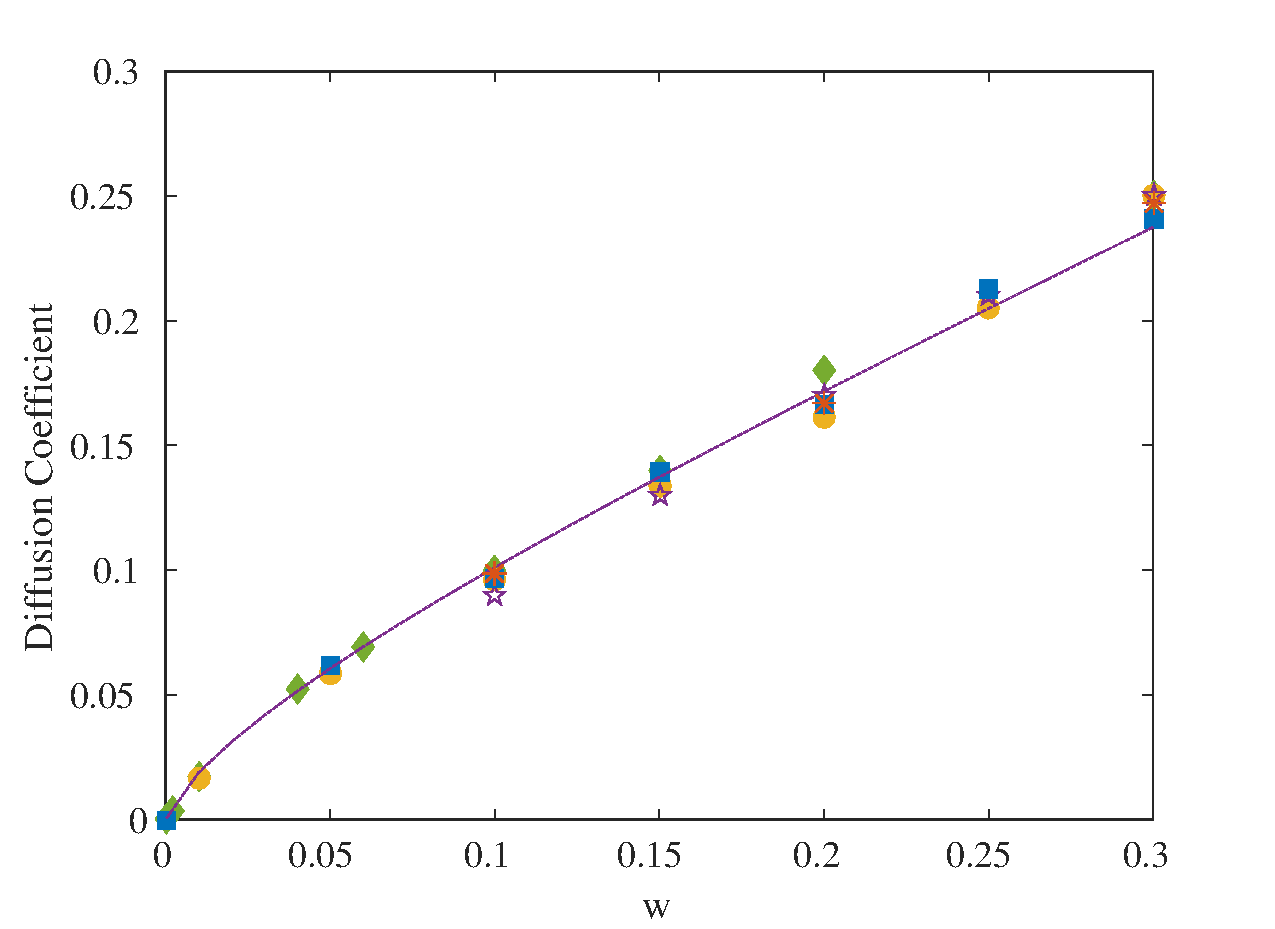
\includegraphics[width=0.45\textwidth]{diffuseDiffCoefPlot}
  \caption[]{\label{fig-results} Diffusion coefficients as a function
  $w$.  Figure generated using data from various resources. Diamonds are
  results from  Green-Kubo numerical experiments\rf{MacZwa83};
  stars\rf{BaEvCo93} and  circles\rf{GasBar95} are calculated from escape
  rate; and triangles are  given by Hausdorff fractal dimension
  calculation\rf{GasBar95}; dashed line  is a statistical
  approximation\rf{Angstmann20121819}}.
\end{figure}

       \TZ{2015-10-19}{Any comment on caption of \reffig{fig-convergence}?}
Compared with various methods, the symmetry reduced cycle expansion
method converges the fastest, table \ref{TCELL2} and
\reffig{fig-convergence}. Diffusion coefficient computed from $\sim2000$
fundamental domain cycles of topological length up to 6 gives two
significant digits, while the elementary cell calculation needs over
$\sim 10000$ cycles in order to converge. In other words, the fundamental
domain cycles suggests a better and denser partition of the phase space.
    \TZ{2015-10-19}{Talk about other two methods}.

To further test \refeq{eq-meanSquareDisp}, we compute the diffusion
coefficient for $w/r = 0.05, 0.10, 0.15, 0.20, 0.25, 0.30$, and compare
the results with existing numerical experiments and a recent statistical
estimation, \reffig{fig-results}. In Green-Kubol velocity
auto-correlation method the  diffusion coefficient can be extrapolated to
the accurate reference value $0.250$ (at $w/r=0.30$), using ensembles of
$10^6\sim10^7$ gas particles flying for long time $T>20$ (and the number
of bounces is greater than this)\rf{MacZwa83}. On the other hand, while
statistical approach yields a smooth analytical
formula\rf{Angstmann20121819}, the diffusion property is fundamentally
never a smooth, monotonically increasing function of $w$
    \TZ{2015-11-02}
    {what is that 1D diffusion reference that shows the anywhere
    continuous, nowhere smooth curve?}
Again, the effectiveness (yet correctness) of the cycle expansion is
proved by those comparison.
